% =====================================================================
\chapter{Comparando famílias de funções}\label{cap:10}
\naaula{37 a 40}

Até aqui, encontramos custos constantes, logarítmicos, lineares, quadráticos, exponenciais e
fatoriais. Este capítulo coloca todos lado a lado e mostra, com números, por que a
\textbf{família} de uma função importa mais do que qualquer constante ou qualquer computador.

\section{A hierarquia}

\begin{center}
\colorbox{edtealclaro}{\large\quad $1 \;<\; \log n \;<\; \sqrt{n} \;<\; n \;<\; n \log n \;<\; n^2 \;<\; n^3 \;<\; 2^n \;<\; n!$\quad}
\end{center}

Leia \enquote{$<$} como \enquote{cresce mais devagar que}, para $n$ grande. Cada família tem
representantes que você já conhece:

\begin{center}
\begin{tabularx}{\textwidth}{P{2.4cm} P{2.8cm} L}
\cab \tc{Família} & \tc{Nome} & \tc{Exemplo} \\
$1$ & constante & \codigo{consultar_topo()}, \codigo{obter(pos)} na lista contígua \\
\rowcolor{edfundo} $\log n$ & logarítmica & adivinhar um número dividindo ao meio; busca binária \\
$\sqrt{n}$ & raiz & busca por saltos em vetor ordenado (capítulo 11) \\
\rowcolor{edfundo} $n$ & linear & \codigo{buscar()}, \codigo{percorrer()}, achar o maior valor \\
$n \log n$ & \enquote{n log n} & os melhores algoritmos de ordenação, como o \codigo{sort()} do Python \\
\rowcolor{edfundo} $n^2$ & quadrática & Insertion Sort no pior caso, interseção ingênua de conjuntos \\
$n^3$ & cúbica & três laços aninhados até $n$ \\
\rowcolor{edfundo} $2^n$ & exponencial & testar todos os subconjuntos de um Conjunto \\
$n!$ & fatorial & testar todas as ordens possíveis de uma fila \\
\end{tabularx}
\end{center}

\section{Os números}

A tabela abaixo foi gerada pelo programa \codigo{python/crescimento_funcoes.py}. Números enormes
aparecem em notação científica: $1{,}3 \times 10^{30}$ quer dizer 1,3 seguido de 30 casas.

\begin{center}
\begin{tabularx}{\textwidth}{P{2.1cm} C C C C C}
\cab \tc{Função} & \tcx{$n = 10$} & \tcx{$n = 20$} & \tcx{$n = 50$} & \tcx{$n = 100$} & \tcx{$n = 1.000$} \\
$\log_2 n$ & 3,3 & 4,3 & 5,6 & 6,6 & 10,0 \\
\rowcolor{edfundo} $\sqrt{n}$ & 3,2 & 4,5 & 7,1 & 10,0 & 31,6 \\
$n$ & 10 & 20 & 50 & 100 & 1.000 \\
\rowcolor{edfundo} $n \log_2 n$ & 33,2 & 86,4 & 282,2 & 664,4 & 9.966 \\
$n^2$ & 100 & 400 & 2.500 & 10.000 & 1.000.000 \\
\rowcolor{edfundo} $n^3$ & 1.000 & 8.000 & 125.000 & 1.000.000 & $1{,}0 \times 10^{9}$ \\
$2^n$ & 1.024 & 1.048.576 & $1{,}1 \times 10^{15}$ & $1{,}3 \times 10^{30}$ & $1{,}1 \times 10^{301}$ \\
\rowcolor{edfundo} $n!$ & 3.628.800 & $2{,}4 \times 10^{18}$ & $3{,}0 \times 10^{64}$ & $9{,}3 \times 10^{157}$ & $4{,}0 \times 10^{2567}$ \\

\end{tabularx}
\end{center}

\begin{intuicao}
Um número como $4{,}0 \times 10^{2567}$ (o valor de $1.000!$) não tem comparação com nada no
mundo real: estima-se que o universo inteiro tenha cerca de $10^{80}$ átomos.
\end{intuicao}

\section{Lendo um gráfico em escala logarítmica}

Se desenharmos essas funções num gráfico comum, $n!$ e $2^n$ disparam para fora da página e as
outras parecem grudadas no chão. A solução é a \textbf{escala logarítmica} no eixo vertical: cada
marca vale 10 vezes (ou mais) a anterior. Assim, números muito diferentes cabem no mesmo desenho.

\begin{figure}[!htb]
  \centering
  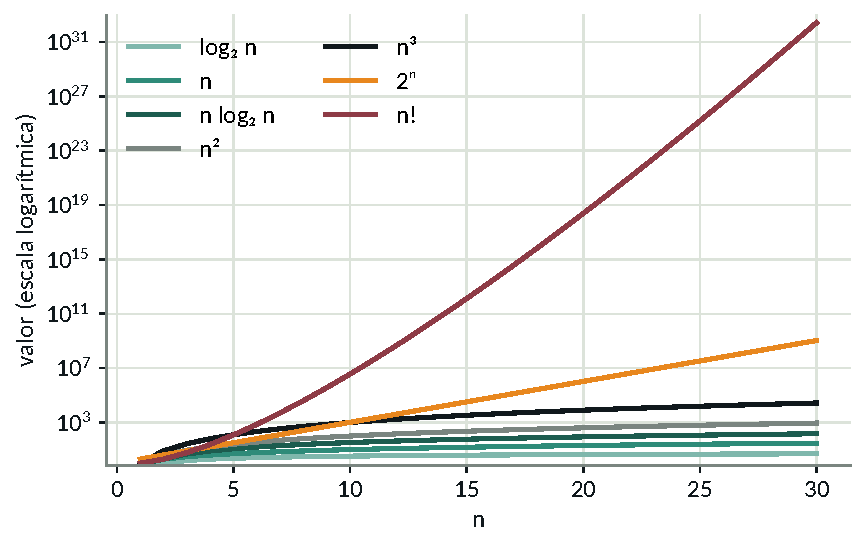
\includegraphics[width=0.76\textwidth]{figuras/f10_familias_log.pdf}
  \caption{As famílias em escala logarítmica. Cada marca do eixo vertical é $10^4$ vezes a
  anterior. $n!$ e $2^n$ se afastam de todas as outras.}
\end{figure}

\begin{atencao}
Numa escala logarítmica, curvas que parecem próximas podem estar muito distantes. A distância
vertical entre duas marcas vizinhas, aqui, é uma multiplicação por 10.000.
\end{atencao}

\section{Transformando em tempo}

Suponha um computador que execute um passo a cada nanossegundo (um bilionésimo de segundo),
ou seja, um bilhão de passos por segundo. Quanto tempo leva cada família?

\begin{center}
\begin{tabularx}{\textwidth}{P{2.1cm} C C C C}
\cab \tc{Passos} & \tcx{$n = 10$} & \tcx{$n = 20$} & \tcx{$n = 50$} & \tcx{$n = 100$} \\
$n$ & 10 ns & 20 ns & 50 ns & 100 ns \\
\rowcolor{edfundo} $n^2$ & 100 ns & 400 ns & 2,5 µs & 10,0 µs \\
$n^3$ & 1,0 µs & 8,0 µs & 125,0 µs & 1,0 ms \\
\rowcolor{edfundo} $2^n$ & 1,0 µs & 1,0 ms & 13 dias & $4{,}0 \times 10^{13}$ anos \\
$n!$ & 3,6 ms & 77 anos & $9{,}6 \times 10^{47}$ anos & $3{,}0 \times 10^{141}$ anos \\

\end{tabularx}
\end{center}
{\small ns = nanossegundo; µs = microssegundo (mil ns); ms = milissegundo (um milhão de ns).
Para comparar: a idade do universo é de cerca de $1{,}4 \times 10^{10}$ anos.}

Com $n = 100$, um algoritmo cúbico termina em 1 milissegundo; um exponencial levaria
$4 \times 10^{13}$ anos — milhares de vezes a idade do universo.

\section{E um computador mil vezes mais rápido?}

É tentador pensar que hardware melhor resolve tudo. Veja o maior $n$ que cabe em 1 segundo hoje
($10^9$ passos) e numa máquina 1.000 vezes mais rápida ($10^{12}$ passos):

\begin{center}
\begin{tabularx}{\textwidth}{P{2.1cm} C C L}
\cab \tc{Passos} & \tc{Maior n hoje} & \tc{Maior n, 1.000× mais rápido} & \tc{Ganho} \\
$n$ & $1{,}0 \times 10^{9}$ & $1{,}0 \times 10^{12}$ & 1.000 vezes maior \\
\rowcolor{edfundo} $n \log_2 n$ & $4{,}0 \times 10^{7}$ & $2{,}9 \times 10^{10}$ & 726 vezes maior \\
$n^2$ & 31.622 & 1.000.000 & 31{,}6 vezes maior \\
\rowcolor{edfundo} $n^3$ & 1.000 & 10.000 & 10{,}0 vezes maior \\
$2^n$ & 29 & 39 & só $+10$ \\
\rowcolor{edfundo} $n!$ & 12 & 14 & só $+2$ \\

\end{tabularx}
\end{center}

Para um algoritmo linear, a máquina nova resolve problemas 1.000 vezes maiores. Para um
quadrático, só 31,6 vezes maiores. Para um exponencial, o ganho é de \textbf{10 elementos}; para
um fatorial, de \textbf{2}. A moral:

\begin{center}
\colorbox{edlaranjaclaro}{\parbox{0.9\textwidth}{\centering\large
Trocar de computador multiplica a velocidade por uma constante.\\
Trocar de algoritmo pode mudar a família — e isso vale muito mais.}}
\end{center}

\begin{exrapido}
Ordene da que cresce mais devagar para a que cresce mais rápido:
$n^2$, $2^n$, $n \log n$, $100$, $n!$, $\sqrt{n}$, $n^3$, $\log n$.
\end{exrapido}

\begin{exrapido}
Um algoritmo exponencial ($2^n$ passos) leva 1 segundo para $n = 30$. (a) Quanto tempo leva para
$n = 31$? (b) E para $n = 40$? (c) Se o algoritmo fosse quadrático ($n^2$ passos) e levasse
1 segundo para $n = 30$, quanto levaria para $n = 40$?
\end{exrapido}

\begin{respostas}
  \resp{10.1} $100 < \log n < \sqrt{n} < n \log n < n^2 < n^3 < 2^n < n!$.
  \resp{10.2} (a) 2 segundos: cada $+1$ em $n$ dobra o tempo. (b) São 10 dobras:
  $2^{10} = 1.024$ segundos, cerca de 17 minutos. (c) O tempo cresce como $(40/30)^2 = 16/9$:
  cerca de 1,8 segundo.
\end{respostas}
